\documentclass[1p]{elsarticle_modified}
%\bibliographystyle{elsarticle-num}

%\usepackage[colorlinks]{hyperref}
%\usepackage{abbrmath_seonhwa} %\Abb, \Ascr, \Acal ,\Abf, \Afrak
\usepackage{amsfonts}
\usepackage{amssymb}
\usepackage{amsmath}
\usepackage{amsthm}
\usepackage{scalefnt}
\usepackage{amsbsy}
\usepackage{kotex}
\usepackage{caption}
\usepackage{subfig}
\usepackage{color}
\usepackage{graphicx}
\usepackage{xcolor} %% white, black, red, green, blue, cyan, magenta, yellow
\usepackage{float}
\usepackage{setspace}
\usepackage{hyperref}

\usepackage{tikz}
\usetikzlibrary{arrows}

\usepackage{multirow}
\usepackage{array} % fixed length table
\usepackage{hhline}

%%%%%%%%%%%%%%%%%%%%%
\makeatletter
\renewcommand*\env@matrix[1][\arraystretch]{%
	\edef\arraystretch{#1}%
	\hskip -\arraycolsep
	\let\@ifnextchar\new@ifnextchar
	\array{*\c@MaxMatrixCols c}}
\makeatother %https://tex.stackexchange.com/questions/14071/how-can-i-increase-the-line-spacing-in-a-matrix
%%%%%%%%%%%%%%%

\usepackage[normalem]{ulem}

\newcommand{\msout}[1]{\ifmmode\text{\sout{\ensuremath{#1}}}\else\sout{#1}\fi}
%SOURCE: \msout is \stkout macro in https://tex.stackexchange.com/questions/20609/strikeout-in-math-mode

\newcommand{\cancel}[1]{
	\ifmmode
	{\color{red}\msout{#1}}
	\else
	{\color{red}\sout{#1}}
	\fi
}

\newcommand{\add}[1]{
	{\color{blue}\uwave{#1}}
}

\newcommand{\replace}[2]{
	\ifmmode
	{\color{red}\msout{#1}}{\color{blue}\uwave{#2}}
	\else
	{\color{red}\sout{#1}}{\color{blue}\uwave{#2}}
	\fi
}

\newcommand{\Sol}{\mathcal{S}} %segment
\newcommand{\D}{D} %diagram
\newcommand{\A}{\mathcal{A}} %arc


%%%%%%%%%%%%%%%%%%%%%%%%%%%%%5 test

\def\sl{\operatorname{\textup{SL}}(2,\Cbb)}
\def\psl{\operatorname{\textup{PSL}}(2,\Cbb)}
\def\quan{\mkern 1mu \triangleright \mkern 1mu}

\theoremstyle{definition}
\newtheorem{thm}{Theorem}[section]
\newtheorem{prop}[thm]{Proposition}
\newtheorem{lem}[thm]{Lemma}
\newtheorem{ques}[thm]{Question}
\newtheorem{cor}[thm]{Corollary}
\newtheorem{defn}[thm]{Definition}
\newtheorem{exam}[thm]{Example}
\newtheorem{rmk}[thm]{Remark}
\newtheorem{alg}[thm]{Algorithm}

\newcommand{\I}{\sqrt{-1}}
\begin{document}

%\begin{frontmatter}
%
%\title{Boundary parabolic representations of knots up to 8 crossings}
%
%%% Group authors per affiliation:
%\author{Yunhi Cho} 
%\address{Department of Mathematics, University of Seoul, Seoul, Korea}
%\ead{yhcho@uos.ac.kr}
%
%
%\author{Seonhwa Kim} %\fnref{s_kim}}
%\address{Center for Geometry and Physics, Institute for Basic Science, Pohang, 37673, Korea}
%\ead{ryeona17@ibs.re.kr}
%
%\author{Hyuk Kim}
%\address{Department of Mathematical Sciences, Seoul National University, Seoul 08826, Korea}
%\ead{hyukkim@snu.ac.kr}
%
%\author{Seokbeom Yoon}
%\address{Department of Mathematical Sciences, Seoul National University, Seoul, 08826,  Korea}
%\ead{sbyoon15@snu.ac.kr}
%
%\begin{abstract}
%We find all boundary parabolic representation of knots up to 8 crossings.
%
%\end{abstract}
%\begin{keyword}
%    \MSC[2010] 57M25 
%\end{keyword}
%
%\end{frontmatter}

%\linenumbers
%\tableofcontents
%
\newcommand\colored[1]{\textcolor{white}{\rule[-0.35ex]{0.8em}{1.4ex}}\kern-0.8em\color{red} #1}%
%\newcommand\colored[1]{\textcolor{white}{ #1}\kern-2.17ex	\textcolor{white}{ #1}\kern-1.81ex	\textcolor{white}{ #1}\kern-2.15ex\color{red}#1	}

{\Large $\underline{12a_{0549}~(K12a_{0549})}$}

\setlength{\tabcolsep}{10pt}
\renewcommand{\arraystretch}{1.6}
\vspace{1cm}\begin{tabular}{m{100pt}>{\centering\arraybackslash}m{274pt}}
\multirow{5}{120pt}{
	\centering
	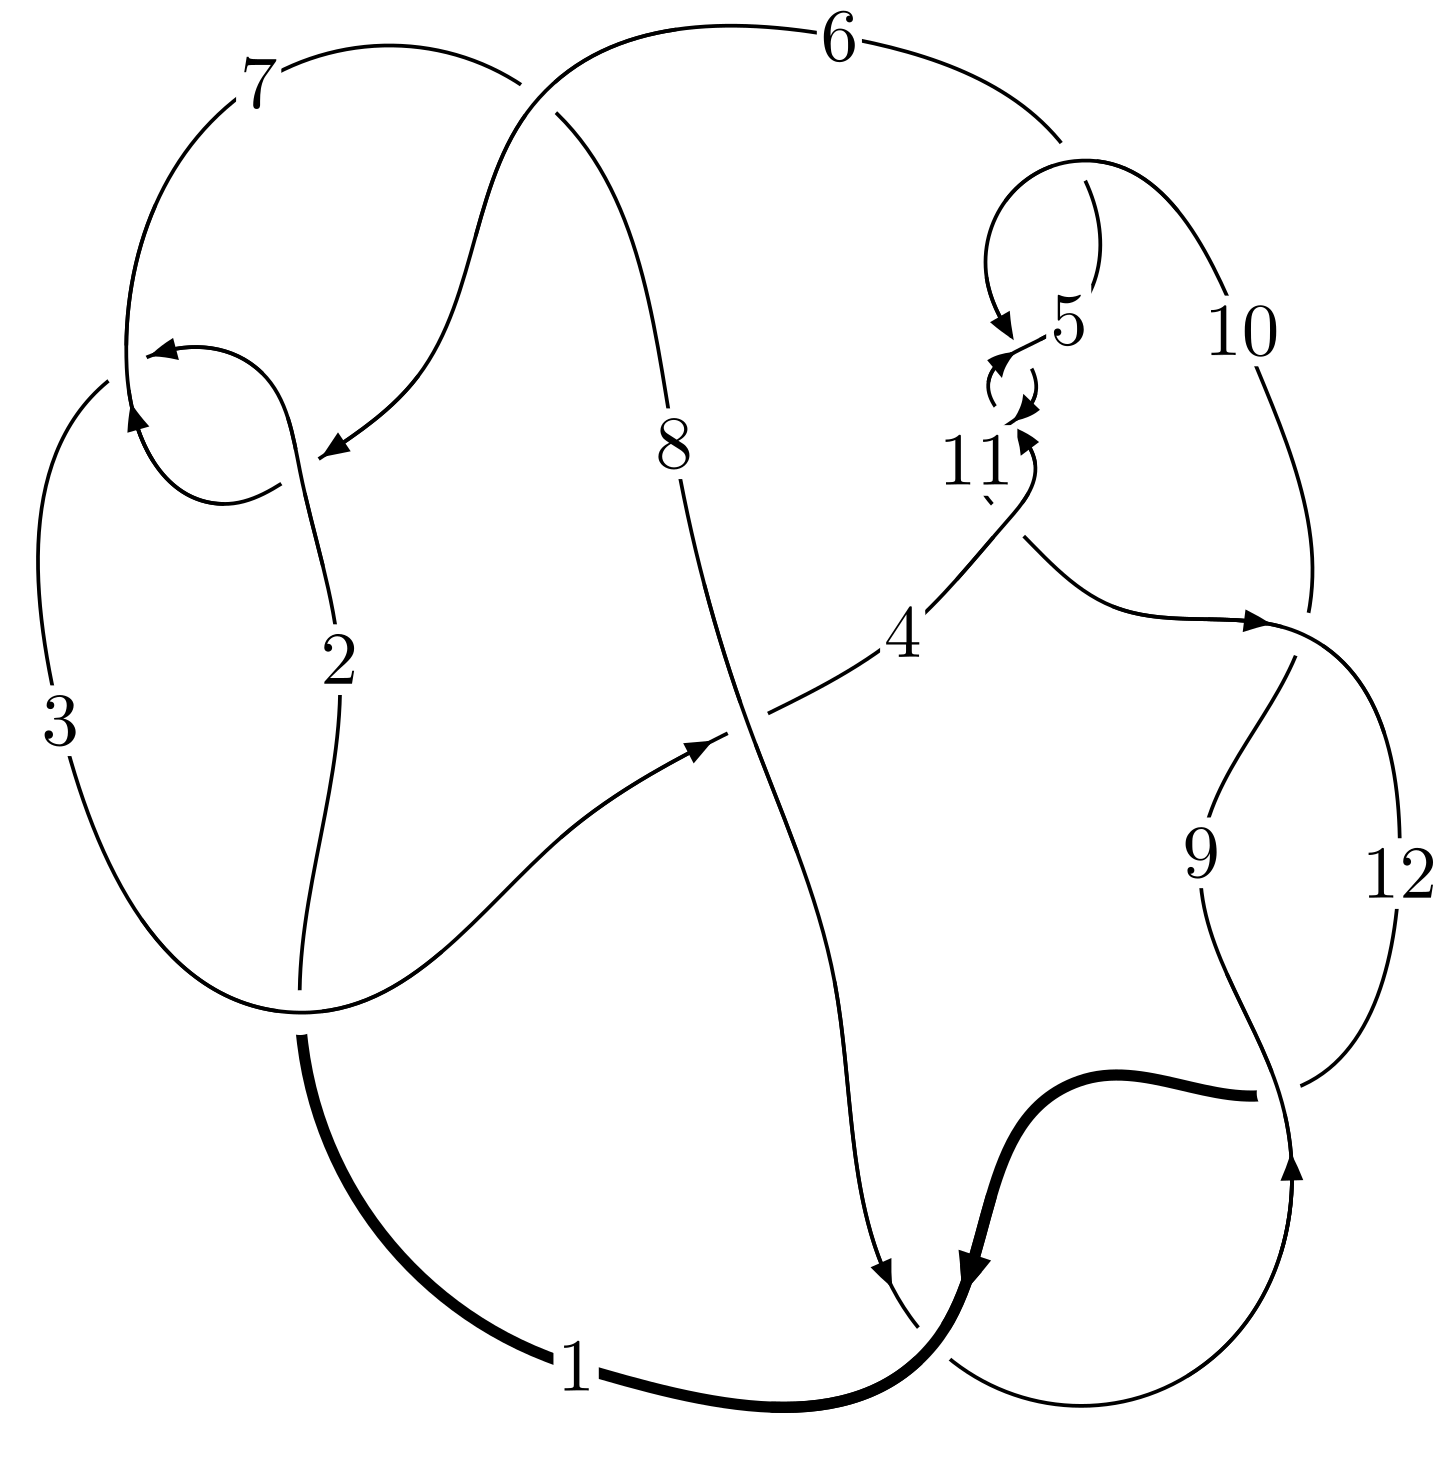
\includegraphics[width=112pt]{../../../GIT/diagram.site/Diagrams/png/1350_12a_0549.png}\\
\ \ \ A knot diagram\footnotemark}&
\allowdisplaybreaks
\textbf{Linearized knot diagam} \\
\cline{2-2}
 &
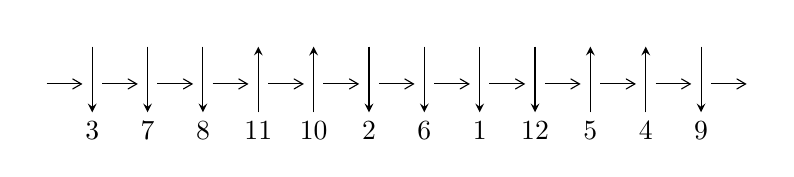
\begin{tikzpicture}[x=20pt, y=17pt]
	% nodes
	\node (C0) at (0, 0) {};
	\node (C1) at (1, 0) {};
	\node (C1U) at (1, +1) {};
	\node (C1D) at (1, -1) {3};

	\node (C2) at (2, 0) {};
	\node (C2U) at (2, +1) {};
	\node (C2D) at (2, -1) {7};

	\node (C3) at (3, 0) {};
	\node (C3U) at (3, +1) {};
	\node (C3D) at (3, -1) {8};

	\node (C4) at (4, 0) {};
	\node (C4U) at (4, +1) {};
	\node (C4D) at (4, -1) {11};

	\node (C5) at (5, 0) {};
	\node (C5U) at (5, +1) {};
	\node (C5D) at (5, -1) {10};

	\node (C6) at (6, 0) {};
	\node (C6U) at (6, +1) {};
	\node (C6D) at (6, -1) {2};

	\node (C7) at (7, 0) {};
	\node (C7U) at (7, +1) {};
	\node (C7D) at (7, -1) {6};

	\node (C8) at (8, 0) {};
	\node (C8U) at (8, +1) {};
	\node (C8D) at (8, -1) {1};

	\node (C9) at (9, 0) {};
	\node (C9U) at (9, +1) {};
	\node (C9D) at (9, -1) {12};

	\node (C10) at (10, 0) {};
	\node (C10U) at (10, +1) {};
	\node (C10D) at (10, -1) {5};

	\node (C11) at (11, 0) {};
	\node (C11U) at (11, +1) {};
	\node (C11D) at (11, -1) {4};

	\node (C12) at (12, 0) {};
	\node (C12U) at (12, +1) {};
	\node (C12D) at (12, -1) {9};
	\node (C13) at (13, 0) {};

	% arrows
	\draw[->,>={angle 60}]
	(C0) edge (C1) (C1) edge (C2) (C2) edge (C3) (C3) edge (C4) (C4) edge (C5) (C5) edge (C6) (C6) edge (C7) (C7) edge (C8) (C8) edge (C9) (C9) edge (C10) (C10) edge (C11) (C11) edge (C12) (C12) edge (C13) ;	\draw[->,>=stealth]
	(C1U) edge (C1D) (C2U) edge (C2D) (C3U) edge (C3D) (C4D) edge (C4U) (C5D) edge (C5U) (C6U) edge (C6D) (C7U) edge (C7D) (C8U) edge (C8D) (C9U) edge (C9D) (C10D) edge (C10U) (C11D) edge (C11U) (C12U) edge (C12D) ;
	\end{tikzpicture} \\
\hhline{~~} \\& 
\textbf{Solving Sequence} \\ \cline{2-2} 
 &
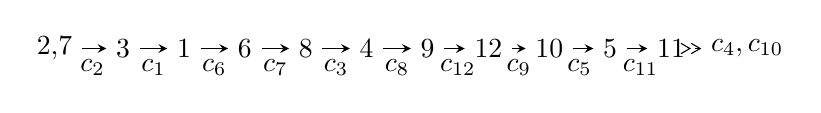
\begin{tikzpicture}[x=22pt, y=7pt]
	% node
	\node (A0) at (-1/8, 0) {2,7};
	\node (A1) at (1, 0) {3};
	\node (A2) at (2, 0) {1};
	\node (A3) at (3, 0) {6};
	\node (A4) at (4, 0) {8};
	\node (A5) at (5, 0) {4};
	\node (A6) at (6, 0) {9};
	\node (A7) at (7, 0) {12};
	\node (A8) at (8, 0) {10};
	\node (A9) at (9, 0) {5};
	\node (A10) at (10, 0) {11};
	\node (C1) at (1/2, -1) {$c_{2}$};
	\node (C2) at (3/2, -1) {$c_{1}$};
	\node (C3) at (5/2, -1) {$c_{6}$};
	\node (C4) at (7/2, -1) {$c_{7}$};
	\node (C5) at (9/2, -1) {$c_{3}$};
	\node (C6) at (11/2, -1) {$c_{8}$};
	\node (C7) at (13/2, -1) {$c_{12}$};
	\node (C8) at (15/2, -1) {$c_{9}$};
	\node (C9) at (17/2, -1) {$c_{5}$};
	\node (C10) at (19/2, -1) {$c_{11}$};
	\node (A11) at (45/4, 0) {$c_{4},c_{10}$};

	% edge
	\draw[->,>=stealth]	
	(A0) edge (A1) (A1) edge (A2) (A2) edge (A3) (A3) edge (A4) (A4) edge (A5) (A5) edge (A6) (A6) edge (A7) (A7) edge (A8) (A8) edge (A9) (A9) edge (A10) ;
	\draw[->>,>={angle 60}]	
	(A10) edge (A11);
\end{tikzpicture} \\ 

\end{tabular} \\

\footnotetext{
The image of knot diagram is generated by the software ``\textbf{Draw programme}" developed by Andrew Bartholomew(\url{http://www.layer8.co.uk/maths/draw/index.htm\#Running-draw}), where we modified some parts for our purpose(\url{https://github.com/CATsTAILs/LinksPainter}).
}\phantom \\ \newline 
\centering \textbf{Ideals for irreducible components\footnotemark of $X_{\text{par}}$} 
 
\begin{align*}
I^u_{1}&=\langle 
u^{55}+u^{54}+\cdots-2 u^2-1\rangle \\
\\
\end{align*}
\raggedright * 1 irreducible components of $\dim_{\mathbb{C}}=0$, with total 55 representations.\\
\footnotetext{All coefficients of polynomials are rational numbers. But the coefficients are sometimes approximated in decimal forms when there is not enough margin.}
\newpage
\renewcommand{\arraystretch}{1}
\centering \section*{I. $I^u_{1}= \langle u^{55}+u^{54}+\cdots-2 u^2-1 \rangle$}
\flushleft \textbf{(i) Arc colorings}\\
\begin{tabular}{m{7pt} m{180pt} m{7pt} m{180pt} }
\flushright $a_{2}=$&$\begin{pmatrix}1\\0\end{pmatrix}$ \\
\flushright $a_{7}=$&$\begin{pmatrix}0\\u\end{pmatrix}$ \\
\flushright $a_{3}=$&$\begin{pmatrix}1\\u^2\end{pmatrix}$ \\
\flushright $a_{1}=$&$\begin{pmatrix}- u^2+1\\- u^4\end{pmatrix}$ \\
\flushright $a_{6}=$&$\begin{pmatrix}u\\u\end{pmatrix}$ \\
\flushright $a_{8}=$&$\begin{pmatrix}- u^3\\- u^3+u\end{pmatrix}$ \\
\flushright $a_{4}=$&$\begin{pmatrix}- u^8+u^6- u^4+1\\- u^8+2 u^6-2 u^4+2 u^2\end{pmatrix}$ \\
\flushright $a_{9}=$&$\begin{pmatrix}- u^9+2 u^7-3 u^5+2 u^3- u\\- u^{11}+u^9-2 u^7+u^5- u^3+u\end{pmatrix}$ \\
\flushright $a_{12}=$&$\begin{pmatrix}- u^{16}+3 u^{14}-7 u^{12}+10 u^{10}-11 u^8+8 u^6-4 u^4+1\\- u^{18}+2 u^{16}-5 u^{14}+6 u^{12}-7 u^{10}+6 u^8-4 u^6+2 u^4- u^2\end{pmatrix}$ \\
\flushright $a_{10}=$&$\begin{pmatrix}- u^{23}+4 u^{21}+\cdots+4 u^3-2 u\\- u^{25}+3 u^{23}+\cdots-3 u^5+u\end{pmatrix}$ \\
\flushright $a_{5}=$&$\begin{pmatrix}u^{49}-8 u^{47}+\cdots-6 u^3+u\\u^{51}-7 u^{49}+\cdots+3 u^3+u\end{pmatrix}$ \\
\flushright $a_{11}=$&$\begin{pmatrix}u^{34}-5 u^{32}+\cdots+3 u^2+1\\u^{34}-6 u^{32}+\cdots+8 u^4- u^2\end{pmatrix}$\\&\end{tabular}
\flushleft \textbf{(ii) Obstruction class $= -1$}\\~\\
\flushleft \textbf{(iii) Cusp Shapes $= -4 u^{53}+32 u^{51}+\cdots+8 u-2$}\\~\\
\newpage\renewcommand{\arraystretch}{1}
\flushleft \textbf{(iv) u-Polynomials at the component}\newline \\
\begin{tabular}{m{50pt}|m{274pt}}
Crossings & \hspace{64pt}u-Polynomials at each crossing \\
\hline $$\begin{aligned}c_{1},c_{7}\end{aligned}$$&$\begin{aligned}
&u^{55}+17 u^{54}+\cdots-4 u+1
\end{aligned}$\\
\hline $$\begin{aligned}c_{2},c_{6}\end{aligned}$$&$\begin{aligned}
&u^{55}- u^{54}+\cdots+2 u^2+1
\end{aligned}$\\
\hline $$\begin{aligned}c_{3}\end{aligned}$$&$\begin{aligned}
&u^{55}+u^{54}+\cdots+1762 u+481
\end{aligned}$\\
\hline $$\begin{aligned}c_{4},c_{5},c_{10}\\c_{11}\end{aligned}$$&$\begin{aligned}
&u^{55}- u^{54}+\cdots+2 u^2+1
\end{aligned}$\\
\hline $$\begin{aligned}c_{8},c_{9},c_{12}\end{aligned}$$&$\begin{aligned}
&u^{55}-7 u^{54}+\cdots+16 u-1
\end{aligned}$\\
\hline
\end{tabular}\\~\\
\newpage\renewcommand{\arraystretch}{1}
\flushleft \textbf{(v) Riley Polynomials at the component}\newline \\
\begin{tabular}{m{50pt}|m{274pt}}
Crossings & \hspace{64pt}Riley Polynomials at each crossing \\
\hline $$\begin{aligned}c_{1},c_{7}\end{aligned}$$&$\begin{aligned}
&y^{55}+43 y^{54}+\cdots-36 y-1
\end{aligned}$\\
\hline $$\begin{aligned}c_{2},c_{6}\end{aligned}$$&$\begin{aligned}
&y^{55}-17 y^{54}+\cdots-4 y-1
\end{aligned}$\\
\hline $$\begin{aligned}c_{3}\end{aligned}$$&$\begin{aligned}
&y^{55}+19 y^{54}+\cdots-1037728 y-231361
\end{aligned}$\\
\hline $$\begin{aligned}c_{4},c_{5},c_{10}\\c_{11}\end{aligned}$$&$\begin{aligned}
&y^{55}+59 y^{54}+\cdots-4 y-1
\end{aligned}$\\
\hline $$\begin{aligned}c_{8},c_{9},c_{12}\end{aligned}$$&$\begin{aligned}
&y^{55}+55 y^{54}+\cdots-164 y-1
\end{aligned}$\\
\hline
\end{tabular}\\~\\
\newpage\flushleft \textbf{(vi) Complex Volumes and Cusp Shapes}
$$\begin{array}{c|c|c}  
\text{Solutions to }I^u_{1}& \I (\text{vol} + \sqrt{-1}CS) & \text{Cusp shape}\\
 \hline 
\begin{aligned}
u &= -0.684404 + 0.722826 I\end{aligned}
 & -5.13814 - 3.11006 I & -5.81726 + 2.62133 I \\ \hline\begin{aligned}
u &= -0.684404 - 0.722826 I\end{aligned}
 & -5.13814 + 3.11006 I & -5.81726 - 2.62133 I \\ \hline\begin{aligned}
u &= \phantom{-}1.009300 + 0.073798 I\end{aligned}
 & -10.64290 - 3.13922 I & -13.9620 + 3.8860 I \\ \hline\begin{aligned}
u &= \phantom{-}1.009300 - 0.073798 I\end{aligned}
 & -10.64290 + 3.13922 I & -13.9620 - 3.8860 I \\ \hline\begin{aligned}
u &= -0.983021 + 0.286921 I\end{aligned}
 & -3.79770 - 1.90653 I & -7.83144 - 0.75410 I \\ \hline\begin{aligned}
u &= -0.983021 - 0.286921 I\end{aligned}
 & -3.79770 + 1.90653 I & -7.83144 + 0.75410 I \\ \hline\begin{aligned}
u &= \phantom{-}0.999075 + 0.254898 I\end{aligned}
 & \phantom{-}2.64629 - 0.91628 I & -4.31373 + 0.57035 I \\ \hline\begin{aligned}
u &= \phantom{-}0.999075 - 0.254898 I\end{aligned}
 & \phantom{-}2.64629 + 0.91628 I & -4.31373 - 0.57035 I \\ \hline\begin{aligned}
u &= \phantom{-}0.739817 + 0.722754 I\end{aligned}
 & \phantom{-}1.96614 + 1.46324 I & -2.76292 - 4.72881 I \\ \hline\begin{aligned}
u &= \phantom{-}0.739817 - 0.722754 I\end{aligned}
 & \phantom{-}1.96614 - 1.46324 I & -2.76292 + 4.72881 I \\ \hline\begin{aligned}
u &= -0.954223 + 0.074852 I\end{aligned}
 & -3.31630 + 2.07955 I & -12.7480 - 6.4347 I \\ \hline\begin{aligned}
u &= -0.954223 - 0.074852 I\end{aligned}
 & -3.31630 - 2.07955 I & -12.7480 + 6.4347 I \\ \hline\begin{aligned}
u &= -1.016950 + 0.234947 I\end{aligned}
 & \phantom{-}2.48031 + 5.10996 I & -4.99601 - 6.99986 I \\ \hline\begin{aligned}
u &= -1.016950 - 0.234947 I\end{aligned}
 & \phantom{-}2.48031 - 5.10996 I & -4.99601 + 6.99986 I \\ \hline\begin{aligned}
u &= \phantom{-}1.033440 + 0.219903 I\end{aligned}
 & -4.29762 - 8.00514 I & -8.76672 + 6.36477 I \\ \hline\begin{aligned}
u &= \phantom{-}1.033440 - 0.219903 I\end{aligned}
 & -4.29762 + 8.00514 I & -8.76672 - 6.36477 I \\ \hline\begin{aligned}
u &= -0.801281 + 0.723501 I\end{aligned}
 & \phantom{-}3.03409 + 1.48960 I & \phantom{-}1.90395 - 3.20693 I \\ \hline\begin{aligned}
u &= -0.801281 - 0.723501 I\end{aligned}
 & \phantom{-}3.03409 - 1.48960 I & \phantom{-}1.90395 + 3.20693 I \\ \hline\begin{aligned}
u &= -0.917815 + 0.588074 I\end{aligned}
 & -7.81316 + 2.22017 I & -10.28022 - 2.96610 I \\ \hline\begin{aligned}
u &= -0.917815 - 0.588074 I\end{aligned}
 & -7.81316 - 2.22017 I & -10.28022 + 2.96610 I \\ \hline\begin{aligned}
u &= \phantom{-}0.882338 + 0.642245 I\end{aligned}
 & -0.37050 - 2.49264 I & -9.18106 + 2.41749 I \\ \hline\begin{aligned}
u &= \phantom{-}0.882338 - 0.642245 I\end{aligned}
 & -0.37050 + 2.49264 I & -9.18106 - 2.41749 I \\ \hline\begin{aligned}
u &= -0.728948 + 0.842191 I\end{aligned}
 & \phantom{-}2.71025 - 7.42439 I & -2.34426 + 3.09843 I \\ \hline\begin{aligned}
u &= -0.728948 - 0.842191 I\end{aligned}
 & \phantom{-}2.71025 + 7.42439 I & -2.34426 - 3.09843 I \\ \hline\begin{aligned}
u &= \phantom{-}0.739346 + 0.840551 I\end{aligned}
 & \phantom{-}9.51060 + 4.33514 I & \phantom{-}1.19741 - 3.41520 I \\ \hline\begin{aligned}
u &= \phantom{-}0.739346 - 0.840551 I\end{aligned}
 & \phantom{-}9.51060 - 4.33514 I & \phantom{-}1.19741 + 3.41520 I \\ \hline\begin{aligned}
u &= -0.749884 + 0.838519 I\end{aligned}
 & \phantom{-}9.70470 + 0.07498 I & \phantom{-}1.76041 - 2.66320 I \\ \hline\begin{aligned}
u &= -0.749884 - 0.838519 I\end{aligned}
 & \phantom{-}9.70470 - 0.07498 I & \phantom{-}1.76041 + 2.66320 I \\ \hline\begin{aligned}
u &= \phantom{-}0.762609 + 0.836176 I\end{aligned}
 & \phantom{-}3.32526 - 3.17260 I & -1.67375 + 2.71266 I \\ \hline\begin{aligned}
u &= \phantom{-}0.762609 - 0.836176 I\end{aligned}
 & \phantom{-}3.32526 + 3.17260 I & -1.67375 - 2.71266 I\\
 \hline 
 \end{array}$$\newpage$$\begin{array}{c|c|c}  
\text{Solutions to }I^u_{1}& \I (\text{vol} + \sqrt{-1}CS) & \text{Cusp shape}\\
 \hline 
\begin{aligned}
u &= \phantom{-}0.862743\phantom{ +0.000000I}\end{aligned}
 & -1.53248\phantom{ +0.000000I} & -4.68320\phantom{ +0.000000I} \\ \hline\begin{aligned}
u &= \phantom{-}0.869677 + 0.749943 I\end{aligned}
 & -1.90030 - 2.83935 I & -4.00000 + 2.97844 I \\ \hline\begin{aligned}
u &= \phantom{-}0.869677 - 0.749943 I\end{aligned}
 & -1.90030 + 2.83935 I & -4.00000 - 2.97844 I \\ \hline\begin{aligned}
u &= -0.925150 + 0.708021 I\end{aligned}
 & \phantom{-}2.65530 + 3.98543 I & \phantom{-0.000000 } 0 \\ \hline\begin{aligned}
u &= -0.925150 - 0.708021 I\end{aligned}
 & \phantom{-}2.65530 - 3.98543 I & \phantom{-0.000000 } 0 \\ \hline\begin{aligned}
u &= \phantom{-}0.960379 + 0.699146 I\end{aligned}
 & \phantom{-}1.30494 - 6.91372 I & \phantom{-0.000000 -}0. + 9.95647 I \\ \hline\begin{aligned}
u &= \phantom{-}0.960379 - 0.699146 I\end{aligned}
 & \phantom{-}1.30494 + 6.91372 I & \phantom{-0.000000 } 0. - 9.95647 I \\ \hline\begin{aligned}
u &= -0.982922 + 0.687300 I\end{aligned}
 & -6.01523 + 8.51848 I & \phantom{-0.000000 } 0 \\ \hline\begin{aligned}
u &= -0.982922 - 0.687300 I\end{aligned}
 & -6.01523 - 8.51848 I & \phantom{-0.000000 } 0 \\ \hline\begin{aligned}
u &= \phantom{-}0.984888 + 0.763099 I\end{aligned}
 & \phantom{-}2.63960 - 2.80293 I & \phantom{-0.000000 } 0 \\ \hline\begin{aligned}
u &= \phantom{-}0.984888 - 0.763099 I\end{aligned}
 & \phantom{-}2.63960 + 2.80293 I & \phantom{-0.000000 } 0 \\ \hline\begin{aligned}
u &= -0.993364 + 0.758698 I\end{aligned}
 & \phantom{-}8.95425 + 5.89271 I & \phantom{-0.000000 } 0 \\ \hline\begin{aligned}
u &= -0.993364 - 0.758698 I\end{aligned}
 & \phantom{-}8.95425 - 5.89271 I & \phantom{-0.000000 } 0 \\ \hline\begin{aligned}
u &= \phantom{-}0.999972 + 0.755227 I\end{aligned}
 & \phantom{-}8.70798 - 10.29670 I & \phantom{-0.000000 } 0 \\ \hline\begin{aligned}
u &= \phantom{-}0.999972 - 0.755227 I\end{aligned}
 & \phantom{-}8.70798 + 10.29670 I & \phantom{-0.000000 } 0 \\ \hline\begin{aligned}
u &= -1.005970 + 0.751628 I\end{aligned}
 & \phantom{-}1.85795 + 13.37800 I & \phantom{-0.000000 } 0 \\ \hline\begin{aligned}
u &= -1.005970 - 0.751628 I\end{aligned}
 & \phantom{-}1.85795 - 13.37800 I & \phantom{-0.000000 } 0 \\ \hline\begin{aligned}
u &= -0.045198 + 0.671804 I\end{aligned}
 & -0.81085 + 5.10342 I & -1.92119 - 3.21301 I \\ \hline\begin{aligned}
u &= -0.045198 - 0.671804 I\end{aligned}
 & -0.81085 - 5.10342 I & -1.92119 + 3.21301 I \\ \hline\begin{aligned}
u &= \phantom{-}0.014665 + 0.668100 I\end{aligned}
 & \phantom{-}5.79986 - 2.14204 I & \phantom{-}1.76494 + 3.28212 I \\ \hline\begin{aligned}
u &= \phantom{-}0.014665 - 0.668100 I\end{aligned}
 & \phantom{-}5.79986 + 2.14204 I & \phantom{-}1.76494 - 3.28212 I \\ \hline\begin{aligned}
u &= -0.311643 + 0.483803 I\end{aligned}
 & -6.70011 + 1.72964 I & -5.80955 - 3.62114 I \\ \hline\begin{aligned}
u &= -0.311643 - 0.483803 I\end{aligned}
 & -6.70011 - 1.72964 I & -5.80955 + 3.62114 I \\ \hline\begin{aligned}
u &= \phantom{-}0.173894 + 0.333363 I\end{aligned}
 & -0.101545 - 0.883584 I & -2.35912 + 7.80336 I \\ \hline\begin{aligned}
u &= \phantom{-}0.173894 - 0.333363 I\end{aligned}
 & -0.101545 + 0.883584 I & -2.35912 - 7.80336 I\\
 \hline 
 \end{array}$$\newpage
\newpage\renewcommand{\arraystretch}{1}
\centering \section*{ II. u-Polynomials}
\begin{tabular}{m{50pt}|m{274pt}}
Crossings & \hspace{64pt}u-Polynomials at each crossing \\
\hline $$\begin{aligned}c_{1},c_{7}\end{aligned}$$&$\begin{aligned}
&u^{55}+17 u^{54}+\cdots-4 u+1
\end{aligned}$\\
\hline $$\begin{aligned}c_{2},c_{6}\end{aligned}$$&$\begin{aligned}
&u^{55}- u^{54}+\cdots+2 u^2+1
\end{aligned}$\\
\hline $$\begin{aligned}c_{3}\end{aligned}$$&$\begin{aligned}
&u^{55}+u^{54}+\cdots+1762 u+481
\end{aligned}$\\
\hline $$\begin{aligned}c_{4},c_{5},c_{10}\\c_{11}\end{aligned}$$&$\begin{aligned}
&u^{55}- u^{54}+\cdots+2 u^2+1
\end{aligned}$\\
\hline $$\begin{aligned}c_{8},c_{9},c_{12}\end{aligned}$$&$\begin{aligned}
&u^{55}-7 u^{54}+\cdots+16 u-1
\end{aligned}$\\
\hline
\end{tabular}\newpage\renewcommand{\arraystretch}{1}
\centering \section*{ III. Riley Polynomials}
\begin{tabular}{m{50pt}|m{274pt}}
Crossings & \hspace{64pt}Riley Polynomials at each crossing \\
\hline $$\begin{aligned}c_{1},c_{7}\end{aligned}$$&$\begin{aligned}
&y^{55}+43 y^{54}+\cdots-36 y-1
\end{aligned}$\\
\hline $$\begin{aligned}c_{2},c_{6}\end{aligned}$$&$\begin{aligned}
&y^{55}-17 y^{54}+\cdots-4 y-1
\end{aligned}$\\
\hline $$\begin{aligned}c_{3}\end{aligned}$$&$\begin{aligned}
&y^{55}+19 y^{54}+\cdots-1037728 y-231361
\end{aligned}$\\
\hline $$\begin{aligned}c_{4},c_{5},c_{10}\\c_{11}\end{aligned}$$&$\begin{aligned}
&y^{55}+59 y^{54}+\cdots-4 y-1
\end{aligned}$\\
\hline $$\begin{aligned}c_{8},c_{9},c_{12}\end{aligned}$$&$\begin{aligned}
&y^{55}+55 y^{54}+\cdots-164 y-1
\end{aligned}$\\
\hline
\end{tabular}
\vskip 2pc
\end{document}